% %%%%%%%%%%%%%%%%%%%%%%%%%%%%%%%%%%%%%%%%%%%%%%%%%%%%%%%%%%%%%%%%%%%%%%%%%%%%%
% %%%%%%%%%%%%%%%%%%%%%%%%%%%%%%%%%%%%%%%%%%%%%%%%%%%%% Gap Between u_B and u_E
% %%%%%%%%%%%%%%%%%%%%%%%%%%%%%%%%%%%%%%%%%%%%%%%%%%%%%%%%%%%%%%%%%%%%%%%%%%%%%

\chapter{Electromagnetic Energy Gap}
  \label{ch_gap}

\todo{A preliminary search (and asking Bob) has not turned up anyone looking at this before, so it's hard to provide context. }

\todo{In \cref{ch_lifetimes}, we considered the decay of energy from the poloidal mode to the toroidal mode. }

\todo{A natural follow up is, do we see any other weird trends in the distribution of energy? }

\todo{As it turns out, yes! }

\todo{At large \azm, a disparity arises between the energy in the electric field components and the energy in the magnetic field components. This is a bit weird, since we would naively expect the poloidal mode to distribute its energy equally between the electric and magnetic fields, and likewise for the toroidal mode. And, at low \azm and at high frequency, that's what we see. The time-averaged energy in the electric field matches the time-averaged energy in the magnetic field almost exactly. }

\todo{However, at high \azm, that's not the case. On the dayside, where the conductivity is large, the magnetic field tends to hold more energy than the electric field. On the nightside, where conductivity is lower, energy is concentrated in the electric field. }

\todo{The directions of these disparities make sense intuitively. If the conductivity is low, it becomes necessary to build up a larger electric field to indice a current to create a magnetic field. But it's not clear why these effects do not appear when \azm is small. }

\todo{Perhaps relatedly, this gap is most visible in the simulations that are worst at resonating. The high-frequency runs continue to accumulate energy over a large number of oscillations, and their electric and magnetic fields stay pretty well matched. But the low-frequency runs level off pretty fast. And, at high \azm, they level off with a significant mismatch between the energy in the electric field and the energy in the magnetic field. }

\begin{figure}[H]
    \centering
    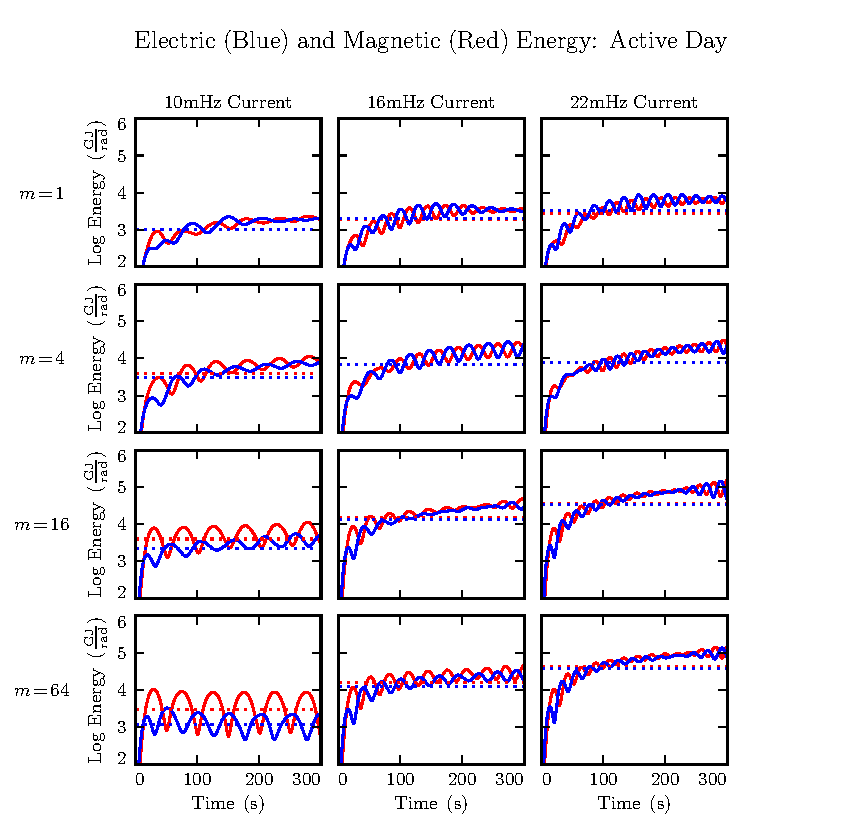
\includegraphics[width=\textwidth]{figures/UB_UE_J_1.pdf}
    \caption[Current-Driven Electric and Magnetic Energy: Active Day]{
      At low \azm, and at high frequency, energy is distributed evenly between the electric and magnetic fields. At low frequency, however, increasing \azm comes with an increasing proportion of the energy in the magnetic field. 
    }
    \label{fig_UB_UE_J_1}
\end{figure}

\begin{figure}[H]
    \centering
    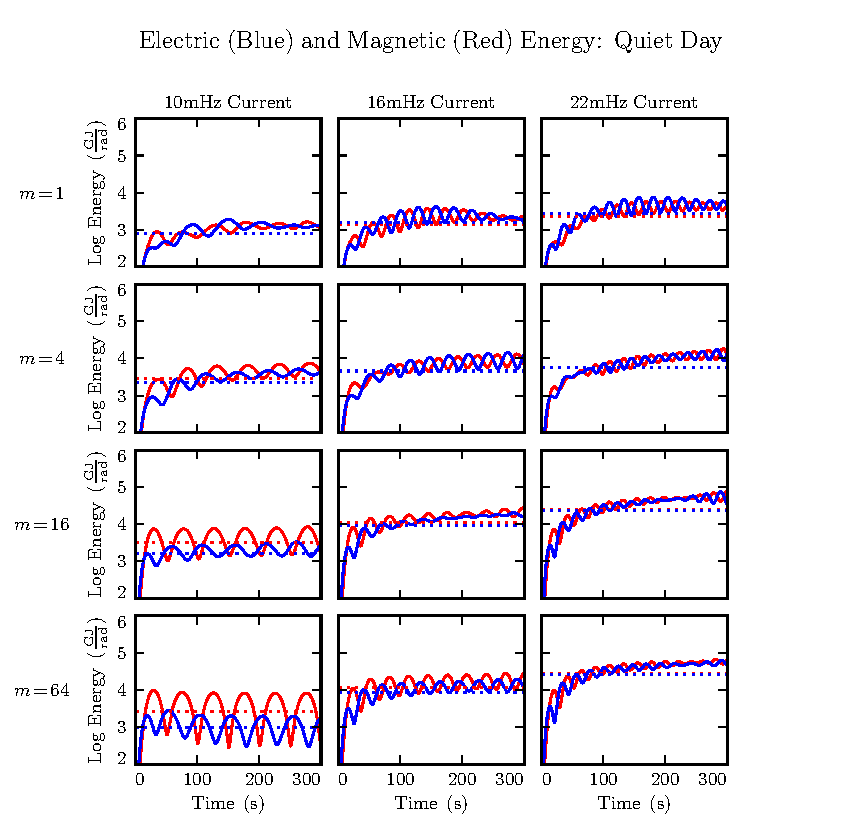
\includegraphics[width=\textwidth]{figures/UB_UE_J_2.pdf}
    \caption[Current-Driven Electric and Magnetic Energy: Quiet Day]{
      As during active times, driving at or above \SI{16}{\mHz} produces no appreciable gap between the energy in the electric field and the energy in the magnetic field. At \SI{10}{\mHz}, the gap becomes increasingly visible as \azm increases. At $\azm = 64$, the magnetic field contains about triple the energy of the magnetic field. 
    }
    \label{fig_UB_UE_J_2}
\end{figure}

\begin{figure}[H]
    \centering
    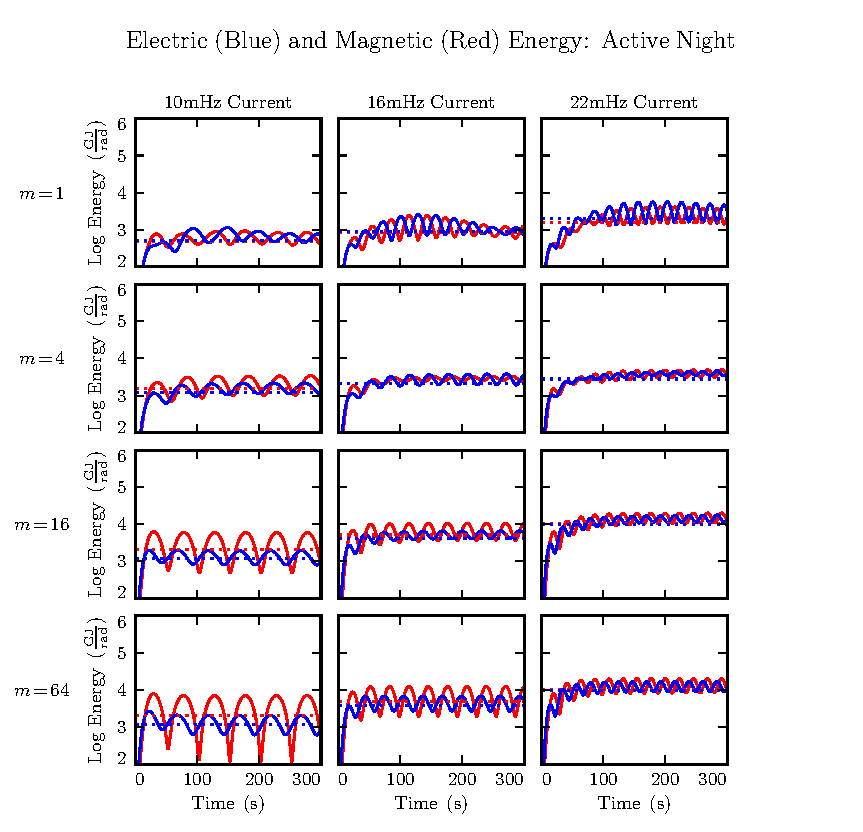
\includegraphics[width=\textwidth]{figures/UB_UE_J_3.pdf}
    \caption[Current-Driven Electric and Magnetic Energy: Active Night]{
      On the nightside, during geomagnetically active times, the gap between the energy in the electric field and the energy in the magnetic field is not particularly prominent. And the dissipation is such that not that much energy builds up anyway. 
    }
    \label{fig_UB_UE_J_3}
\end{figure}

\begin{figure}[H]
    \centering
    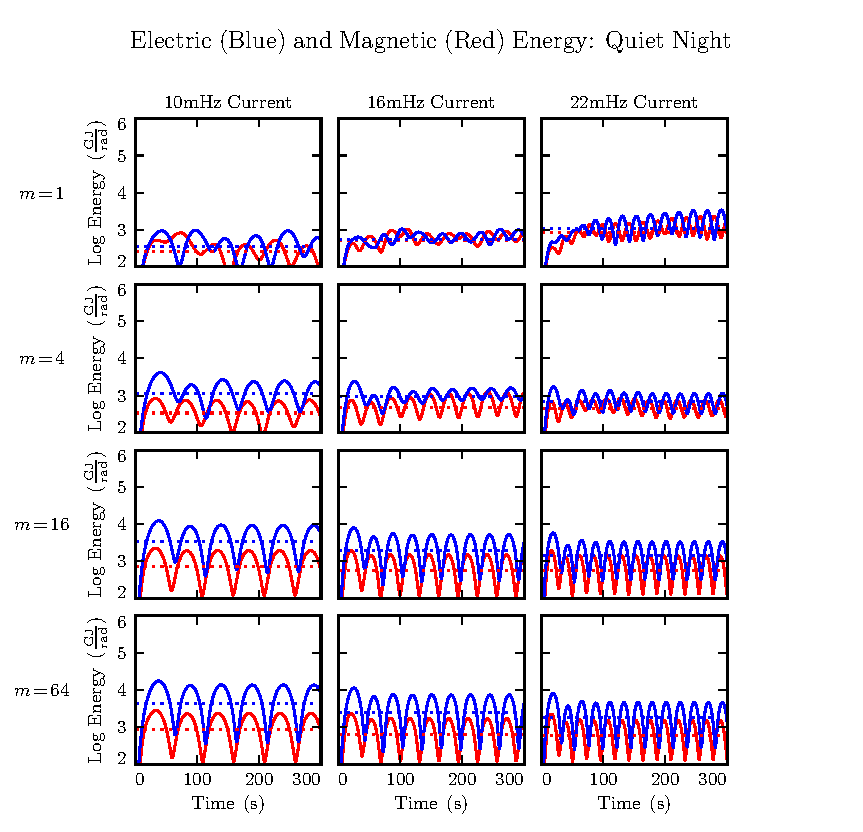
\includegraphics[width=\textwidth]{figures/UB_UE_J_4.pdf}
    \caption[Current-Driven Electric and Magnetic Energy: Quiet Night]{
      In contrast to the tother three profiles, the geomagnetically quiet nightside seems to accumulate energy in the electric field, rather than the magnetic field. This may mean that dissipation is so high that energy doesn't even move effectively out of the driving electric field. Note that \cref{fig_UP_UT_J_4} shows most of the energy in this run remaining in the poloidal mode. 
    }
    \label{fig_UB_UE_J_4}
\end{figure}










